\subsection{Logical Architecture}
\label{sec:logical-architecture}
 
The logical architecture is a high-level view of the application. It describes the technical organization of the code into layers and the software-level data flow across the entire infrastructure. 

The application's logical architecture is designed according to \textbf{Clean Architecture} principles. Its core objective is to separate the responsibilities of each layer. The result is a clean code structure in which business logic and domain rules are independent of external service implementations. As a consequence, the system is highly maintainable, testable, and extensible. Figure \ref{fig:logical-architecture-diagram} depicts the application's logical architecture.

\begin{figure}[H]
    \centering
    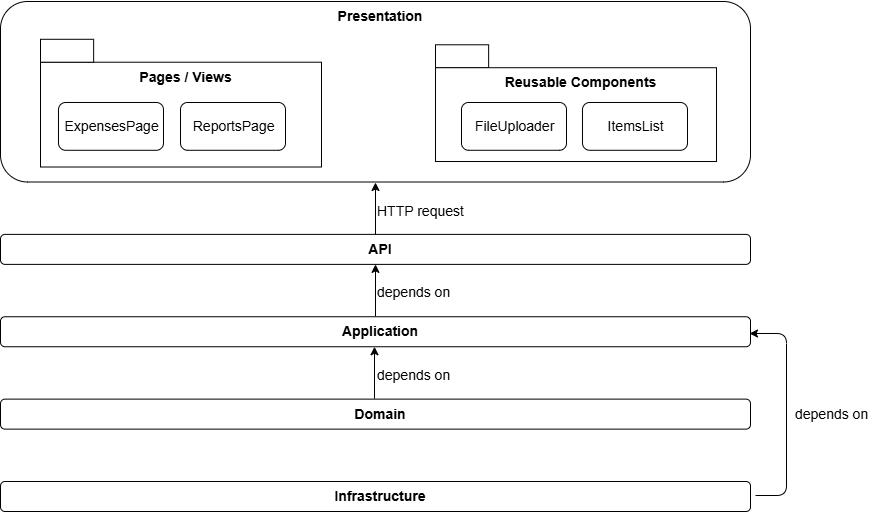
\includegraphics[width=\textwidth]{Images/LogicalArchitecture.png}
    \caption[Logical architecture diagram]
    {Logical architecture diagram. [Own creation]}
    \label{fig:logical-architecture-diagram}
\end{figure}


\subsubsection{Logical Layers}

The application's logical architecture is visually divided into the following main layers:	

\textbf{Presentation layer}

The Presentation layer corresponds to the frontend component and is responsible for handling the user interface, user experience, and API communication. Each navigation state or view in the application corresponds to a distinct page, and each reusable component can be used across multiple pages.

The user interface is built using React with TypeScript. This strategic choice allows developers to leverage React's component-based architecture, enabling the creation of reusable UI blocks (components) that compose larger screens (pages). Although this approach requires a more complex initial implementation effort, it speeds up development and improves code maintainability and extensibility over time. TypeScript also enforces contract definitions, ensuring consistency across the frontend data flow. 

\textbf{API layer}

The API layer exposes the application's use cases to external parties via RESTful HTTP endpoints. Different controllers handle distinct functional areas (set of use cases), with the main controllers dedicated to Expenses and Reports. Controllers receive HTTP requests, validate them, translate them into commands or queries for the Application layer, and return an HTTP response. This layer, along with the subsequent ones, constitutes the backend component and uses the ASP.NET Core platform.

\vspace{1cm}

\textbf{Application Layer}

The Application layer contains the application logic and is responsible for handling all use cases. This layer orchestrates entities defined in the Domain layer to execute business rules and interacts with repository abstractions (interfaces) to retrieve and persist data. The concrete implementations of these repositories are provided by the Infrastructure layer.


Additionally, this layer defines Data Transfer Objects (DTOs) and interfaces. DTOs standardize data exchange between components, while interfaces are abstractions that specify how external dependencies are accessed without exposing implementation details.

\textbf{Domain layer}

The Domain layer is the core of the application and represents the business model. It encapsulates entities (e.g., \texttt{Expense}, \texttt{User}), value objects, and the most critical and stable business rules. This is a pure layer, with no dependencies on other layers, and it remains independent of how data is stored or presented to the user. This independence ensures a stable and long-lasting business model.

\textbf{Infrastructure layer}

While the Application layer depends on abstractions to perform data access and communicate with external services, the Infrastructure layer provides the corresponding concrete implementations. It is responsible for handling communication with external systems and services. \texttt{ExpenseRepository}, \texttt{BlobStorageService}, and \texttt{DocumentIntelligenceService} are some of the implementations contained in this layer.

This layer is expected to evolve as external technologies and infrastructure requirements change. For example, switching from Blob Storage to another storage provider only requires changes within this layer, without affecting the upper layers, which depend on abstractions rather than concrete implementations.

Another key advantage of using the .NET platform is availability of Entity Framework Core (EF Core) and the built-in Dependency Injection (DI) container. EF Core enables higher-level interaction with the database, allowing data manipulation, relationship management, and migrations through clear, easy-to-understand C\texttt{\#} code. DI is explained in more detail in the next section.

\subsubsection{Guiding Principles and Design Patterns}
\label{sec:principles-and-patterns}

The structure described above is not arbitrary; it is intentionally crafted based on a set of industry-standard principles and patterns that ensure high-quality, professional software design. 

\textbf{The SOLID principles}

The SOLID principles are a set of five foundational guidelines that help developers create maintainable and flexible software solutions. This application's architecture adheres to them as follows:

\begin{enumerate} [leftmargin=0.75cm]
    
    \item \textbf{Single Responsibility Principle}
    Each class and layer serves a single purpose and, therefore, has only one reason to change. A clear example is the separation of expense-related responsibilities:

    \begin{itemize} [leftmargin=0.75cm, label=\textbullet]
        
        \item The \texttt{ExpensesController} in the API layer handles HTTP communication with the Presentation layer by receiving requests and returning responses; changes are required only when the API contract evolves.

        \item The \texttt{ExpenseService} in the Application layer is responsible for expense-related business logic; modifications occur only when business rules change.

        \item The \texttt{ExpenseRepository} in the Infrastructure layer manages data persistence; changes are required only when the database or storage service changes.

    \end{itemize}

    \item \textbf{Open/Closed Principle}

    The system is open for extension but closed for modification. Thanks to the interfaces defined in the Application layer, introducing new functionality requires only the implementation of new classes in the Infrastructure layer. The existing, tested code in the Application layer remains unchanged.

    Currently, the \texttt{RepositoryService} in the Application layer depends on the \texttt{IEmailNoti- ficationService}. If, in the future, clients require SMS notifications in addition to email notifications, it is sufficient to introduce a new \texttt{SMSNotificationService} class in the Infrastructure layer that implements a common \texttt{INotificationService} interface. The \texttt{RepositoryService} does not require any modification.

    \item \textbf{Liskov Substitution Principle}

    Any implementation of an interface should be substitutable for another without breaking the application. A clear example is the use of repositories: any class at the Infrastructure layer that implements the \texttt{IExpenseRepository} interface can be used interchangeably by the Application layer. Components that depend on external interfaces are responsible only for knowing how to use them, not for understanding their implementation.

    \item \textbf{Interface Segregation Principle}

    Components should not be forced to depend on unnecessary interfaces. Interfaces are defined at a granular level, such as \texttt{IExpenseRepository} and \texttt{IFileStorage}, rather than combining responsibilities into a single large interface. As a result, components depend only on the interfaces they truly require.

    \item \textbf{Dependency Inversion Principle}

    This is the key principle that holds Clean Architecture together. High-level modules should not depend on low-level modules. For example, the Application layer does not depend on the Infrastructure layer; instead, both depend on abstractions (interfaces). Consequently, as illustrated in Figure \ref{fig:logical-architecture-diagram}, the Infrastructure layer points inward toward the Application layer, resulting in a core business logic that is independent of external concerns.

\end{enumerate}

\textbf{Key Design Patterns}

Several well-known design patterns are used throughout the source code to support the application of these principles:

\begin{itemize} [leftmargin=0.75cm, label=\textbullet]
    
    \item \textbf{Programming to an Interface}

    Components do not depend on concrete classes; instead, they rely on abstract interfaces. These interfaces (e.g., \texttt{IExpenseRepository}) define clear contracts for interacting with external components without exposing services' internal logic. This approach is the primary mechanism for achieving a decoupled system. 

    \item \textbf{Service Pattern}

    The logic in the Application layer is organized into services (e.g., \texttt{ExpenseService}). Each service groups related business operations, providing a clear and easy-to-understand structure. 

    \item \textbf{DTO Pattern}

    Data Transfer Objects (DTOs) are simple data containers that protect internal domain models from external exposure. Their primary purpose is to facilitate data transfer between the API and Application layers, establishing a clear and consistent contract between them. 

    \item \textbf{Domain-Driven Design (DDD)}

    The Domain layer is structured according to Domain-Driven Design principles. It encapsulates the core business logic within a pure, isolated layer.

    \item \textbf{Repository Pattern}

    Repositories implement interfaces such as \texttt{IExpenseRepository} and encapsulate the logic behind these abstractions. For example, the Application layer can request to save an expense via \texttt{IExpenseRepository} without needing to know which database or storage mechanism is used. 

    \item \textbf{Dependency Injection (DI)} 

    Dependency Injection enables components to depend on external sources (e.g., \texttt{Expen- seService} depends on a repository for data operations). It is the practical implementation of the Dependency Inversion Principle, allowing layers to remain decoupled in the code while being connected and functional at runtime. This approach clarifies component responsibilities, reduces the need for code changes, and simplifies testing by removing dependencies on internal implementations. 

\end{itemize}

All these patterns collectively support and reinforce the adoption of Clean Architecture principles. For a complete overview of the system structure applying these principles and patterns, refer to the UML Class Diagram in Section \ref{sec:backend-class-diagram}.

